At room temperatures, the branching ratio has been found to be approximately 84:16 (\ce{COH+}:\ce{HCO+})\cite{Freeman1987}, but unexplored at lower regimes.

To determine the branching ratio, \ce{Be+} and \ce{C+} in the trap are exposed to the CBGB for 10 s, after which, the gate valve connecting the differential pumping region and ion trap chamber is closed. \ce{^15N2} is then introduced via leak valve to react with the \ce{HOC+}. Only runs taken at delay times of 10 s were taken, as we only concern ourselves with a ratio of signals.

\begin{figure}[H]
	\centering
	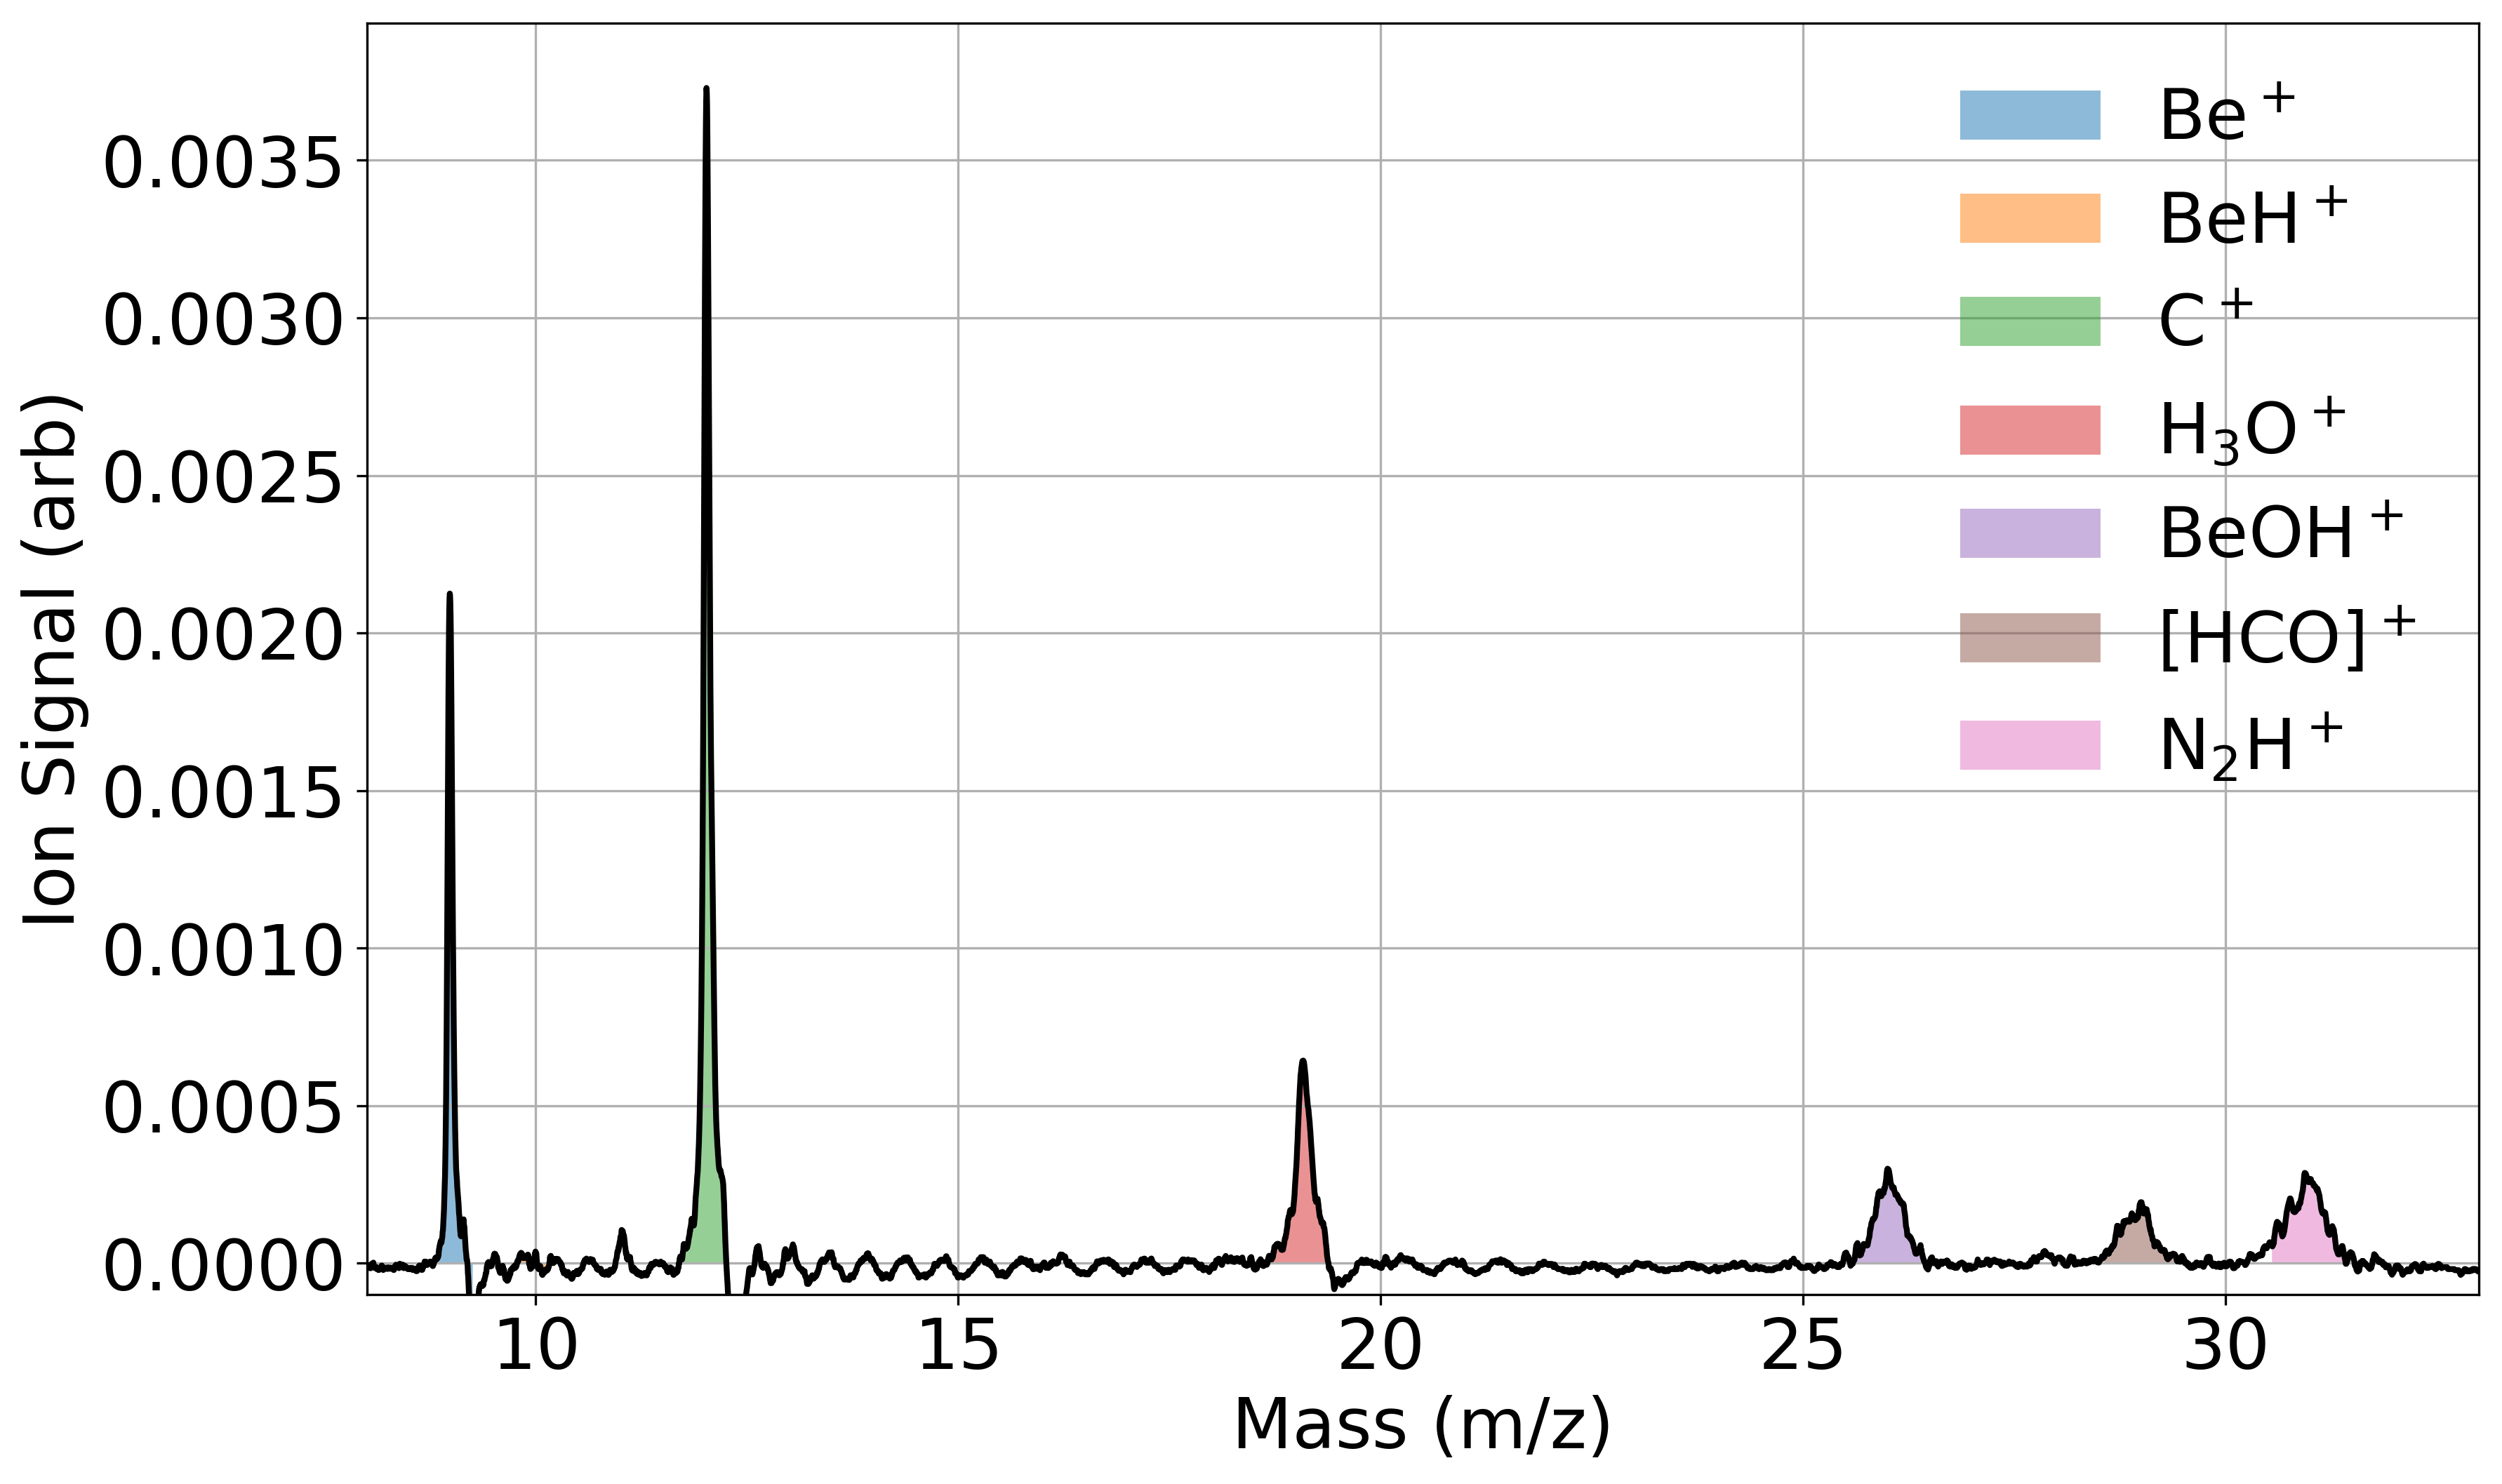
\includegraphics[width=0.8\textwidth]{images/C_H2O_15N2.png}
\end{figure}

Repeating this process over various densities of \ce{^15N2} allows us to determine the isomer branching ratio. We expect the ratio of \ce{N2H+} and \ce{[HCO]+} to follow the form:

\begin{equation}
	\eta(t) = C \left( 1-e^{-k_{\ref{r: X+HOC->XH}} \rho t} \right)
	\label{eq: N2 asymptote}
\end{equation}

Where we define $\eta(t) \equiv \frac{\ce{^{15}N2H+}(t)}{\ce{^{15}N2H+}(t)+\ce{[HCO]+}(t)}$. A fit performed on the data over various densities yields a rate constant of $k_{\ref{r: X+HOC->XH}} = ((6.2 \pm 1.0) \times 10^{-10})$ cm$^3$/s, and a final branching ratio of $\ce{HOC+}:\ce{HCO+} = 0.58 \pm 0.02$.

\begin{figure}[H]
	\centering
	\label{fig: N2 pressure scan}
	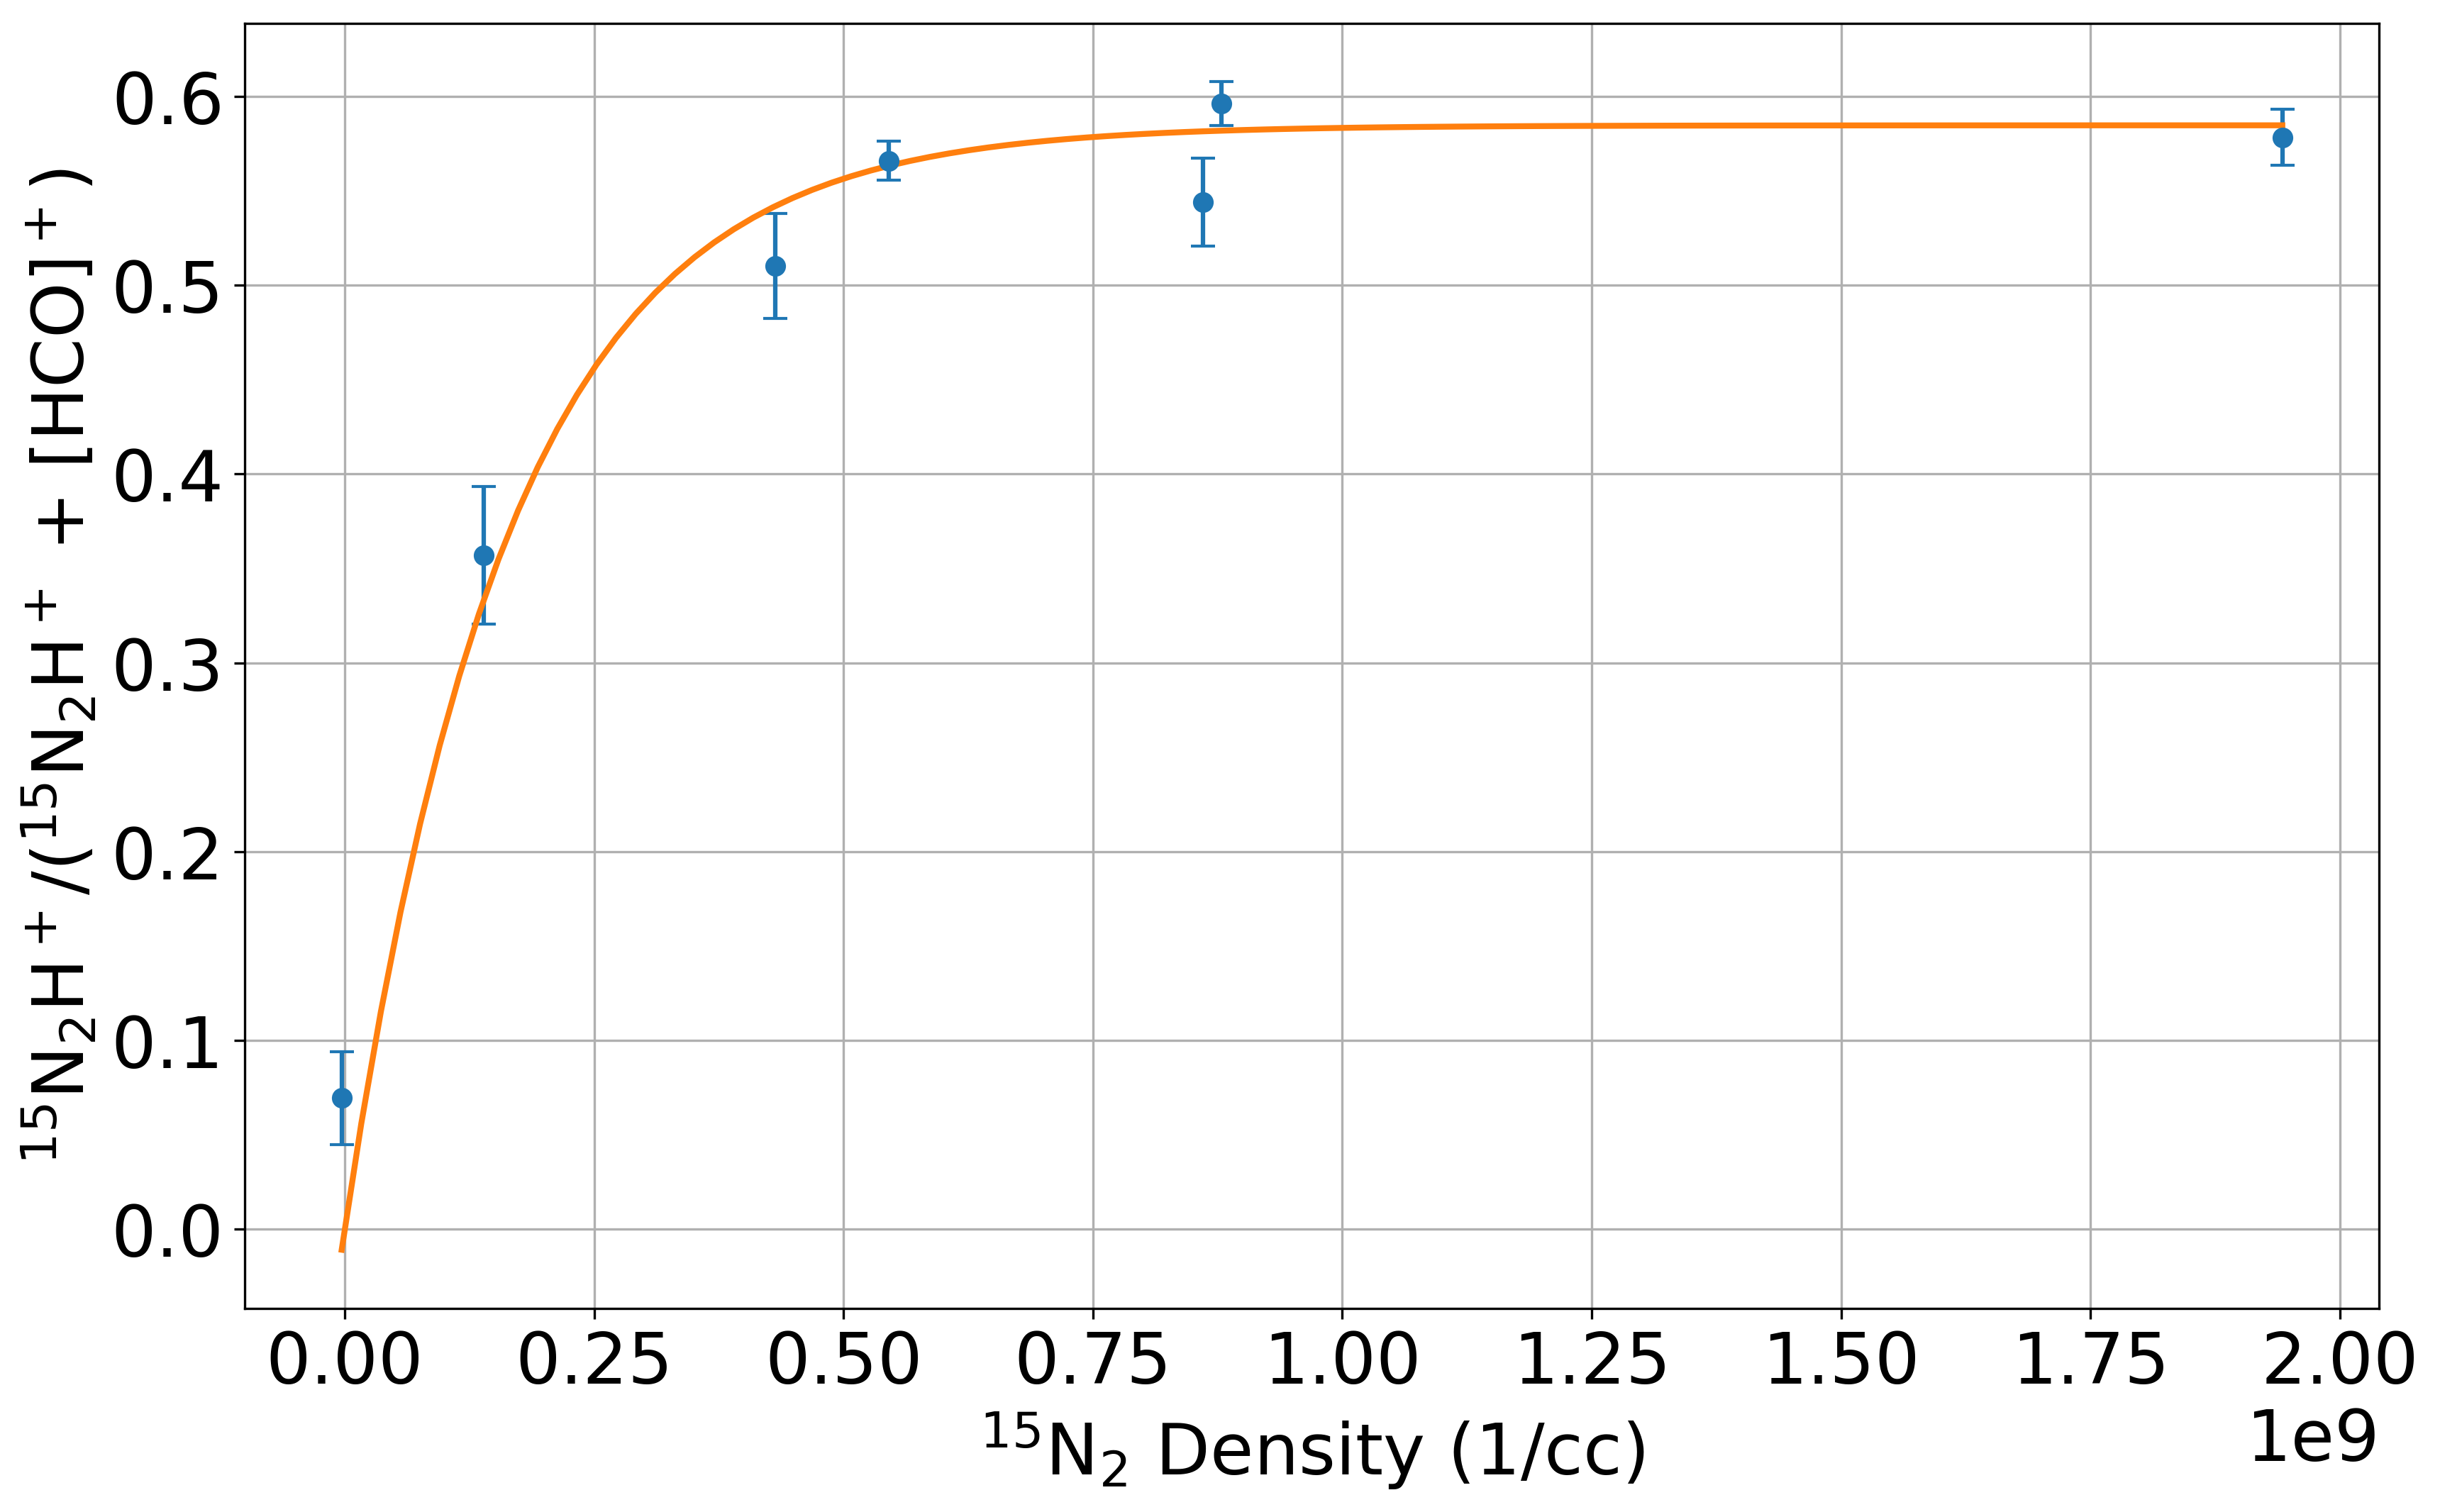
\includegraphics[width=0.8\textwidth]{images/N2_pressure_scan.png}
	\caption{\ce{^15N2} introduced into the ion chamber after trapped \ce{Be+} and \ce{C+} are exposed to water from the CBGB for set times.}
\end{figure}

With this fit, we may consider putting bounds on the rate of isomerization by comparing the theoretical rate constant for reaction \ref{r: X+HOC->XH} with the fitted value. If reaction \ref{r: X+HOC->HCO} plays a role, it will proportionally affect the total rate constant. We find the Langevin rate for \ce{HOC+ + ^15N2} to be $k_L = 8.0 \times 10^{-10}$ cm$^3$/s

To estimate a limit on the isomerization, we consider the above reaction \cref{r: X+HOC->HCO,r: X+HOC->XH}, where \ce{X = ^{15}N2} in the context that we can only determine the abundance of \ce{[HCO]+} and \ce{^{15}N2H+}. As a function of pressure, we cannot see reaction \ref{r: X+HOC->HCO}, but if it does contribute, we should see a discrepancy in the total rate constant, which we estimate to be Langevin: $k_L = 8.0 \times 10^{-10}$. This gives us a possible isomerization rate of 22\%, which then yield a branching ratio of 70:30

%CO with beam
%
%k1: 7.39e-02, 5.88e-03
%k2: 2.23e-01, 2.02e-02
%C0: 8.25e-01, 7.11e-02
%mz290: 9.36e-02, 1.71e-02
%H3O0: 1.75e-02, 3.24e-03
%reduced chi squared: 1.31e+00
%k1 = 7.87e-09
%k2 = 2.38e-08
%k1 theory = 7.74e-09
%k2 theory = 5.15e-09

%beam 
%k1: 2.11e-02, 4.04e-03
%k2: 5.30e-02, 9.73e-03
%C0: 8.49e-01, 1.08e-01
%mz290: 3.52e-02, 9.54e-03
%H3O0: 9.63e-03, 3.12e-03
%reduced chi squared: 2.50e+00
%k1 = 9.14e-09
%k2 = 2.29e-08
%k1 theory = 7.74e-09
%k2 theory = 5.15e-09